%%% The main file. It contains definitions of basic parameters and includes all other parts.

%% Settings for single-side (simplex) printing
% Margins: left 40mm, right 25mm, top and bottom 25mm
% (but beware, LaTeX adds 1in implicitly)
\documentclass[12pt,a4paper]{report}
\setlength\textwidth{145mm}
\setlength\textheight{247mm}
\setlength\oddsidemargin{15mm}
\setlength\evensidemargin{15mm}
\setlength\topmargin{0mm}
\setlength\headsep{0mm}
\setlength\headheight{0mm}
% \openright makes the following text appear on a right-hand page
\let\openright=\clearpage

%% Settings for two-sided (duplex) printing
% \documentclass[12pt,a4paper,twoside,openright]{report}
% \setlength\textwidth{145mm}
% \setlength\textheight{247mm}
% \setlength\oddsidemargin{14.2mm}
% \setlength\evensidemargin{0mm}
% \setlength\topmargin{0mm}
% \setlength\headsep{0mm}
% \setlength\headheight{0mm}
% \let\openright=\cleardoublepage

%% Generate PDF/A-2u
\usepackage[a-2u]{pdfx}

%% Character encoding: usually latin2, cp1250 or utf8:
\usepackage[utf8]{inputenc}

%% Prefer Latin Modern fonts
\usepackage{lmodern}

%% Further useful packages (included in most LaTeX distributions)
\usepackage{amsmath}        % extensions for typesetting of math
\usepackage{amsfonts}       % math fonts
\usepackage{amsthm}         % theorems, definitions, etc.
\usepackage{bbding}         % various symbols (squares, asterisks, scissors, ...)
\usepackage{bm}             % boldface symbols (\bm)
\usepackage{graphicx}       % embedding of pictures
\usepackage{fancyvrb}       % improved verbatim environment
\usepackage{natbib}         % citation style AUTHOR (YEAR), or AUTHOR [NUMBER]
\usepackage[nottoc]{tocbibind} % makes sure that bibliography and the lists
			    % of figures/tables are included in the table
			    % of contents
\usepackage{dcolumn}        % improved alignment of table columns
\usepackage{booktabs}       % improved horizontal lines in tables
\usepackage{paralist}       % improved enumerate and itemize
\usepackage{xcolor}         % typesetting in color

\usepackage{tikz-qtree}

\usetikzlibrary{shapes.geometric}
\tikzset{every tree node/.style={minimum width=2em,draw,circle},
         blank/.style={draw=none},
         edge from parent/.style=
         {draw,edge from parent path={(\tikzparentnode) -- (\tikzchildnode.north)}},
         level distance=1.2cm,
         triangle/.style={regular polygon, regular polygon sides=3}
         }


%%% Basic information on the thesis

% Thesis title in English (exactly as in the formal assignment)
\def\ThesisTitle{Persistent Data Structures Built Upon Weak AVL Trees}

% Author of the thesis
\def\ThesisAuthor{Jiří Škrobánek}

% Year when the thesis is submitted
\def\YearSubmitted{2020}

% Name of the department or institute, where the work was officially assigned
% (according to the Organizational Structure of MFF UK in English,
% or a full name of a department outside MFF)
\def\Department{Department of Applied Mathematics}

% Is it a department (katedra), or an institute (ústav)?
\def\DeptType{Department}

% Thesis supervisor: name, surname and titles
\def\Supervisor{Mgr. Martin Mareš, Ph.D.}

% Supervisor's department (again according to Organizational structure of MFF)
\def\SupervisorsDepartment{Department of Applied Mathematics}

% Study programme and specialization
\def\StudyProgramme{Computer Science}
\def\StudyBranch{General Computer Science}

% An optional dedication: you can thank whomever you wish (your supervisor,
% consultant, a person who lent the software, etc.)
\def\Dedication{%
Dedication.
}

% Abstract (recommended length around 80-200 words; this is not a copy of your thesis assignment!)
\def\Abstract{%
Abstract.
}

% 3 to 5 keywords (recommended), each enclosed in curly braces
\def\Keywords{%
{key} {words}
}

%% The hyperref package for clickable links in PDF and also for storing
%% metadata to PDF (including the table of contents).
%% Most settings are pre-set by the pdfx package.
\hypersetup{unicode}
\hypersetup{breaklinks=true}

% Definitions of macros (see description inside)
%%% This file contains definitions of various useful macros and environments %%%
%%% Please add more macros here instead of cluttering other files with them. %%%

%%% Minor tweaks of style

% These macros employ a little dirty trick to convince LaTeX to typeset
% chapter headings sanely, without lots of empty space above them.
% Feel free to ignore.
\makeatletter
\def\@makechapterhead#1{
  {\parindent \z@ \raggedright \normalfont
   \Huge\bfseries \thechapter. #1
   \par\nobreak
   \vskip 20\p@
}}
\def\@makeschapterhead#1{
  {\parindent \z@ \raggedright \normalfont
   \Huge\bfseries #1
   \par\nobreak
   \vskip 20\p@
}}
\makeatother

% This macro defines a chapter, which is not numbered, but is included
% in the table of contents.
\def\chapwithtoc#1{
\chapter*{#1}
\addcontentsline{toc}{chapter}{#1}
}

% Draw black "slugs" whenever a line overflows, so that we can spot it easily.
\overfullrule=1mm

%%% Macros for definitions, theorems, claims, examples, ... (requires amsthm package)

\newtheoremstyle{mytheoremstyle} % name
{\topsep}                    % Space above
{\topsep}                    % Space below
{\slshape}                   % Body font
{}                           % Indent amount
{\bfseries}                   % Theorem head font
{.}                          % Punctuation after theorem head
{.5em}                       % Space after theorem head
{}  % Theorem head spec (can be left empty, meaning ‘normal’)

\theoremstyle{mytheoremstyle}
\newtheorem{thm}{Theorem}
\newtheorem{lemma}[thm]{Lemma}
\newtheorem{claim}[thm]{Claim}
\newtheorem{prop}[thm]{Proposition}

\theoremstyle{mytheoremstyle}
\newtheorem{defn}{Definition}

\theoremstyle{remark}
\newtheorem*{cor}{Corollary}
\newtheorem*{obs}{Observation}
\newtheorem*{rem}{Remark}
\newtheorem*{example}{Example}

%%% An environment for proofs

\newenvironment{myproof}{
  \par\medskip\noindent
  \textit{Proof}.
}{
\newline
\rightline{$\qedsymbol$}
}

%%% An environment for typesetting of program code and input/output
%%% of programs. (Requires the fancyvrb package -- fancy verbatim.)

\DefineVerbatimEnvironment{code}{Verbatim}{fontsize=\small, frame=single}

%%% The field of all real and natural numbers
\newcommand{\R}{\mathbb{R}}
\newcommand{\N}{\mathbb{N}}

%%% Useful operators for statistics and probability
\DeclareMathOperator{\pr}{\textsf{P}}
\DeclareMathOperator{\E}{\textsf{E}\,}
\DeclareMathOperator{\var}{\textrm{var}}
\DeclareMathOperator{\sd}{\textrm{sd}}

%%% Transposition of a vector/matrix
\newcommand{\T}[1]{#1^\top}

%%% Various math goodies
\newcommand{\goto}{\rightarrow}
\newcommand{\gotop}{\stackrel{P}{\longrightarrow}}
\newcommand{\maon}[1]{o(n^{#1})}
\newcommand{\abs}[1]{\left|{#1}\right|}
\newcommand{\dint}{\int_0^\tau\!\!\int_0^\tau}
\newcommand{\isqr}[1]{\frac{1}{\sqrt{#1}}}

%%% Various table goodies
\newcommand{\pulrad}[1]{\raisebox{1.5ex}[0pt]{#1}}
\newcommand{\mc}[1]{\multicolumn{1}{c}{#1}}

\newcommand{\bigO}[1]{$\mathcal{O}(#1)$}

\newenvironment{vdTable}[1]{
\begin{tabular}{|m{0.085\textwidth} m{0.06\textwidth} m{0.06\textwidth} m{0.06\textwidth} m{0.06\textwidth}|}
\hline
\bfseries #1 & & & & \\
}{
\\ \hline
	\end{tabular}
}

%https://tex.stackexchange.com/questions/12703/how-to-create-fixed-width-table-columns-with-text-raggedright-centered-raggedlef

% Mathmode slanted:

\def\leftit{\text{\it left}}
\def\rightit{\text{\it right}}
\def\sizeit{\text{\it size}}
\def\weightit{\text{\it weight}}
\def\keyit{\text{\it key}}

% Title page and various mandatory informational pages
\begin{document}
%%% Title page of the thesis and other mandatory pages

%%% Title page of the thesis

\pagestyle{empty}
\hypersetup{pageanchor=false}
\begin{center}

\centerline{\mbox{
\includegraphics[width=166mm]{../img/logo-en.pdf}}}

\vspace{-8mm}
\vfill

{\bf\Large BACHELOR THESIS}

\vfill

{\LARGE\ThesisAuthor}

\vspace{15mm}

{\LARGE\bfseries\ThesisTitle}

\vfill

\Department

\vfill

{
\centerline{\vbox{\halign{\hbox to 0.45\hsize{\hfil #}&\hskip 0.5em\parbox[t]{0.45\hsize}{\raggedright #}\cr
Supervisor of the bachelor thesis:&\Supervisor \cr
\noalign{\vspace{2mm}}
Study programme:&\StudyProgramme \cr
\noalign{\vspace{2mm}}
Study branch:&\StudyBranch \cr
}}}}

\vfill

% Zde doplňte rok
Prague \YearSubmitted

\end{center}

\newpage

%%% Here should be a bound sheet included -- a signed copy of the "bachelor
%%% thesis assignment". This assignment is NOT a part of the electronic
%%% version of the thesis. DO NOT SCAN.

%%% A page with a solemn declaration to the bachelor thesis

\openright
\hypersetup{pageanchor=true}
\pagestyle{plain}
\pagenumbering{roman}
\vglue 0pt plus 1fill

\noindent
I declare that I carried out this bachelor thesis independently, and only with the cited
sources, literature and other professional sources. It has not been used to obtain another
or the same degree.

\medskip\noindent
I understand that my work relates to the rights and obligations under the Act No.~121/2000 Sb.,
the Copyright Act, as amended, in particular the fact that the Charles
University has the right to conclude a license agreement on the use of this
work as a school work pursuant to Section 60 subsection 1 of the Copyright~Act.

\vspace{10mm}

\hbox{\hbox to 0.5\hsize{%
In \hbox to 6em{\dotfill} date \hbox to 6em{\dotfill}
\hss}\hbox to 0.5\hsize{\dotfill\quad}}
\smallskip
\hbox{\hbox to 0.5\hsize{}\hbox to 0.5\hsize{\hfil Author's signature\hfil}}

\vspace{20mm}
\newpage

%%% Dedication

\openright

\noindent
\Dedication

\newpage

%%% Mandatory information page of the thesis

\openright

\vbox to 0.5\vsize{
\setlength\parindent{0mm}
\setlength\parskip{5mm}

Title:
\ThesisTitle

Author:
\ThesisAuthor

\DeptType:
\Department

Supervisor:
\Supervisor, \SupervisorsDepartment

Abstract:
\Abstract

Keywords:
\Keywords

\vss}

\newpage

\openright
\pagestyle{plain}
\pagenumbering{arabic}
\setcounter{page}{1}


%%% A page with automatically generated table of contents of the bachelor thesis

\tableofcontents

%%% Each chapter is kept in a separate file
\chapter*{Introduction}
\addcontentsline{toc}{chapter}{Introduction}

Speaking in general terms, persistent data structures maintain their previous versions when modified. Use of term "persistent" was introduced by Driscoll, Sarnak, Sleator, and Tarjan in their joint 1986 article \emph{Making data structures persistent} \cite{persistence-DSST}. In this article a general scheme for converting regular pointer-based data structures into persistent ones is given. Persistent binary search tree was constructed from adapted Red-Black trees.

Haeupler, Sen, and Tarjan \cite{weight-balanced} introduced Weak-AVL (WAVL) trees as part of a framework of rank balanced trees in 2015. WAVL trees were named after AVL trees which form a subset of them.

The algorithms for WAVL operations given by Haeupler at al. cannot be directly plugged into the persistence scheme by Driscoll at al. Modifications will be needed alike those done to red-black trees during their conversion into persistent binary search trees. This thesis aims to construct a persistent version of Weak-AVL trees.

We begin the thesis by swiftly establishing fundamentals of binary search trees. These topics are covered in Chapter 1. Chapter 2 moves to construct our modification of WAVL trees suitable for persistence. Several approaches to persistence of binary search trees are described in Chapter 3. A structure for handling versions as elements of an ordering is also covered. Persistent data structures were motivated by many direct and obscured applications, we mention some of them in Chapter 4. Implementation of persistent WAVL trees is the focus of Chapter 5.

% Since the original publication on persistence great number of other works addressing this topic appeared.

\chapter{Weak AVL Trees}



\section{Original Weak-AVL Tree}

\begin{defn}
A binary tree is said to be {\em ranked binary tree} if all vertices have non-negative integer ranks assigned. External vertices are by convention given rank $-1$. We denote $r(V)$ the rank of vertex $V$.
\end{defn}

\begin{defn}
Vertex $V$ having left child $L$ and right child $R$ (both of which may be external) in ranked binary tree may be said to be either $(a,b)$-vertex or $(b,a)$-vertex if $r(V) - r(L) = a$ and $r(V) - r(R) = b$. $L$ and $R$ are called $a$-child and $b$-child.
\end{defn}

\begin{prop}
Let $S$ be a finite subset of ${(\mathbb{Z} _ +)}^2$ and $T$ a ranked tree with $n$ vertices. If it holds that for every $(i,j)$-vertex in $T$ that $(i,j) \in S$, then the height of $T$ is $\Theta(\log n)$.
\label{thm-rbt-depth}
\end{prop}

\begin{myproof}
Let us denote $m$ the maximum allowed rank difference by $S$.
We prove this by induction on the rank of the root vertex. We establish a lower bound on the number of vertices in a tree with root of rank $r$. 
We suppose that it holds for every lower rank $q$, that the number of vertices in a tree with root of rank $q$ is at least $\exp(qc)$ for some positive constant $c$. 
Then to continue the induction we need the following: $$ 1 + 2\exp((r-m)c) \geq \exp(rc) $$ $$ \log 2 + (r-m)c \geq rc $$ $$ \log 2 \geq cm $$
We see that setting $c$ will be always possible.
The base case of rank zero: The inequality obviously holds for leaves (only possible vertices with rank zero).\\
Then $n \geq \exp(qc)$, if $q$ is the rank of root of $T$. The height of $T$ is in turn at most $ \log(n)/c $. 
The other inclusion applies to all kinds of binary search trees.
\end{myproof}

The theory of ranked trees permits a nice definition of AVL trees\cite{avl}.

\begin{defn}
A ranked tree is said to be {\em AVL tree} if all its every vertex is either $(1,1), (1,2)$ or $(2,1)$  and all leaves are of rank 0.
\end{defn}

The conditions on rank differences are referred to as rank invariants.

\begin{defn}
A ranked tree is said to be {\em Weak-AVL tree} if all its vertices are either $(1,1), (1,2), (2,1)$ or $(2,2)$ and all leaves are of rank 0.
\end{defn}

WAVL trees use a relaxation of the balancing rules of AVL trees, this implies that all Weak-AVL trees form a proper subset AVL trees.

From now on, we will ignore symmetric situations. Only one from the pair of $(a,b)$- $(b,a)$- vertices will be considered.

\subsection{Bottom-up rebalancing}

By default WAVL trees use the set of standard set of operations as outlined earlier with rebalancing that is described in this section. A series of steps is taken until the rank invariants are restored.

% Rebalancing consists of checking rank invariant for vertices on the path from the changed vertex back to the root one by one, while performing balancing steps where needed. 

\subsubsection*{Rebalancing after Insert}

Inserting a new leaf $l$ itself may only introduce one type of violation, making the parent of $l$ into a $(0,1)$- or a $(0,2)$-vertex. It will become apparent that the existence of one $(0,1)$- or $(0,2)$-vertex in the tree is the only violation that may happen during this rebalancing. 

Rebalancing after inserts consists of repeatedly checking the rank invariant for vertex $y$. Where $y$ changes during the rebalancing and takes values from the vertices in the BST. Initially $y$ is the parent of the inserted vertex. 

Once the whole subtree of $y$ respects the rank rules, rebalancing proceeds by setting $y$ to be the parent of current $y$. All descendants of $y$ obviously adhere to rank invariant. Either it was not violated by this operation or it has just been amended. 

There are three balancing steps to rectify rank violation at $y$ after insert. (See figures for better illustration.) If rank invariant does not hold for $y$, one of the following steps is chosen, there are symmetric variants for all of these steps. 

\begin{itemize}
	\item \textbf{Promote} If $y$ is a $(0,1)$-vertex, rank of $y$ is increased by 1. This may make the parent of $y$ a $(0,1)$- or $(0,2)$-vertex. Rebalancing thus continues with the parent of $y$ taking role of $y$. (Unless $y$ is the root, then no additional rebalancing is needed.)
	\item \textbf{Rotate} If $y$ is a (0,2)-vertex and the 0-child $x$ is a (1,1)-vertex, we rotate along the edge $xy$. The rank of $y$ is decremented by 1. Rebalancing ends.
	\item \textbf{Double Rotate} If $y$ is a (0,2)-vertex and the 0-child $x$ is a (2,1)-vertex with the 1-child being $w$, we rotate along the edge $xy$ and then along the edge $xw$. Rebalancing ends.
\end{itemize}

One can easily verify that every case is covered by the outlined steps. Most importantly, if rebalancing continues beyond the first vertex, one child of $y$ must be a $(2,1)$-vertex as one of the children must have been promoted and as such it is a $(2,1)$-vertex. This implies existence of an applicable step. 

At the first checked vertex $v$, one of its children has just been inserted. If $v$ was a leaf, promote can be used. If $v$ had one children prior to this insert, it must have rank 1 and insert may be applied. 

\begin{figure}
\begin{center}
\begin{tikzpicture}[sibling distance=32pt]
\Tree
[ \edge node[auto=right]{1 or 2}; [.$y$
    \edge[tosubtree] node[auto=right] {0};
    \node[draw,triangle]{~};
    \edge[tosubtree] node[auto=left] {1};
    \node[draw,triangle]{~};
] ]
\end{tikzpicture}
\qquad
\begin{tikzpicture}[sibling distance=32pt]
\Tree
[ \edge node[auto=right]{0 or 1}; [.$y$
    \edge[tosubtree] node[auto=right] {1};
    \node[draw,triangle]{~};
    \edge[tosubtree] node[auto=left] {2};
    \node[draw,triangle]{~};
] ]
\end{tikzpicture}
\end{center}
{\small Situation displayed on the left depicts the structure prior to the step and situation on the right after the step. Edges are annotated by rank differences between the endpoint vertices. This convention is followed for depictions of all steps in this section.}
\caption{Promote step}
\end{figure}

\begin{figure}
\begin{center}
\begin{tikzpicture}[sibling distance=32pt, 
	frontier/.style={distance from root=4cm}]
\Tree
[ \edge node[auto=right]{1 or 2}; [.$y$
    \edge node[auto=right] {0};
    [   .$x$ 
        \edge[tosubtree] node[auto=right] {1}; 
        \node[draw,triangle]{A}; 
        \edge[tosubtree] node[auto=left] {2};
        \node[draw,triangle]{B}; ]
    \edge[tosubtree] node[auto=left] {2};
    \node[draw,triangle]{C};
] ]
\end{tikzpicture}
\qquad
\begin{tikzpicture}[sibling distance=32pt, 
	frontier/.style={distance from root=4cm}]
\Tree
[ \edge node[auto=right]{1 or 2}; [.$x$
    \edge[tosubtree] node[auto=right] {1};
    \node[draw,triangle]{A};
    \edge node[auto=left] {1};
    [   .$y$ 
        \edge[tosubtree] node[auto=right] {1}; 
        \node[draw,triangle]{B}; 
        \edge[tosubtree] node[auto=left] {1}; 
        \node[draw,triangle]{C}; ]
] ]
\end{tikzpicture}
\end{center}
\caption{Insert rotation step}
\end{figure}

\begin{figure}.
\begin{center}
\begin{tikzpicture}[sibling distance=8pt, frontier/.style={distance from root=5.25cm}]
\Tree
[ 
    \edge node[auto=right]{1 or 2}; 
    [
        .$y$
        \edge node[auto=right] {0};
        [   
            .$x$ 
            \edge[tosubtree] node[auto=right] {2}; 
            \node[draw,triangle]{A}; 
            \edge node[auto=left] {1};
            [
                .$w$
                \edge[tosubtree]; 
                \node[draw,triangle]{B};
                \edge[tosubtree]; 
                \node[draw,triangle]{C}; 
            ]
        ]
        \edge[tosubtree] node[auto=left] {2};
        \node[draw,triangle]{D};
    ] 
]
\end{tikzpicture}
\qquad
\begin{tikzpicture}[sibling distance=8pt, frontier/.style={distance from root=4cm}]
\Tree
[ \edge node[auto=right]{1 or 2}; [.$w$
    \edge node[auto=right] {1};
    [ 
        .$x$
        \edge[tosubtree] node[auto=right] {1};
        \node[draw,triangle]{A};
        \edge[tosubtree];
        \node[draw,triangle]{B};
    ]
    \edge node[auto=left] {1};
    [   .$y$ 
    	\edge[tosubtree];
        \node[draw,triangle]{C}; 
        \edge[tosubtree] node[auto=left] {1}; 
        \node[draw,triangle]{D}; ]
] ]
\end{tikzpicture}
\end{center}
\caption{Insert double rotation step}
\end{figure}

\subsubsection*{Rebalancing after Delete}

This process is analogous to reblancing after insert in many ways. Deleting a leaf may cause its former parent to become either a $(3,1)$-vertex, a $(3,2)$-vertex, a $(2,2)$-vertex that is a leaf, or a $(2,1)$-vertex. This is easily seen from examining all possibilities. 

Starting from the parent of the deleted vertex, going towards the root, the rank invariant is checked for every vertex $y$ on that path.  During the rebalancing only one vertex may violate the rank invariant at a time and if so, it must either $(3,1)$ or $(3,2)$, (with the exception of the initial $(2,2)$-leaf).

There are four different balancing steps, one of which is applied if the rank invariant does not hold at $y$. (Again, these are illustrated in figures.)
\begin{itemize}
	\item \textbf{Demote} If $y$ is a $(3,2)$-vertex or a $(2,2)$-leaf, the rank of $y$ is decremented by 1 and rebalancing continues with the parent of $y$ taking the role of $y$. (If $y$ is the root, rebalancing ends.)
	\item \textbf{Demote of the Second Kind} If $y$ is a $(3,1)$-vertex and its 1-child is a $(2,2)$-vertex, the rank of $y$ and its 1-child is decremented by 1 and rebalancing continues with the parent of $y$ taking the role of $y$. (If $y$ is the root, rebalancing ends.)
	\item \textbf{Rotate} If $y$ is a $(3,1)$-vertex, the 1-child $x$ is the right child and its right child is 1-child, we rotate along $xy$, decrementing rank of $y$ by 1 and incrementing the rank of $x$. Rebalancing ends. Of course, in the symmetric case when the 1-child is the left child, symmetric changes must be applied.
	\item \textbf{Double Rotate} If $y$ is a $(3,1)$-vertex, the 1-child $x$ is the right child and a $(2,1)$-vertex and also the 2-child $w$ of $x$ is its left child, we rotate along $xy$ and then along $wy$, decrementing rank of $y$ by 2, of $x$ by 1 and incrementing the rank of $w$ by 2. Rebalancing ends. Of course, in the symmetric case when the 1-child is the left child, symmetric changes must be applied.
\end{itemize}

\begin{figure}
	\begin{center}
		\begin{tikzpicture}[sibling distance=32pt]
		\Tree
		[ \edge node[auto=right]{1 or 2}; [.Y
		\edge node[auto=right] {3};
		\node[draw,triangle]{~};
		\edge node[auto=left] {2};
		\node[draw,triangle]{~};
		] ]
		\end{tikzpicture}
		\qquad
		\begin{tikzpicture}[sibling distance=32pt]
		\Tree
		[ \edge node[auto=right]{2 or 3}; [.Y
		\edge node[auto=right] {2};
		\node[draw,triangle]{~};
		\edge node[auto=left] {1};
		\node[draw,triangle]{~};
		] ]
		\end{tikzpicture}
	\end{center}
	\caption{Demote of the first kind step}
\end{figure}


\begin{figure}
	\begin{center}
		\begin{tikzpicture}[sibling distance=8pt, frontier/.style={distance from root=4cm}]
		\Tree[ 
		\edge node[auto=right] {1 or 2};
		[   
		.$x$ 
		\edge[tosubtree] node[auto=right] {3}; 
		\node[draw,triangle]{A}; 
		\edge node[auto=left] {1};
		[
		.$y$
		\edge[tosubtree] node[auto=right] {2};
		\node[draw,triangle]{B};
		\edge[tosubtree] node[auto=left] {2};
		\node[draw,triangle]{C}; 
		] ] ]
		\end{tikzpicture}
		\qquad
		\begin{tikzpicture}[sibling distance=8pt, frontier/.style={distance from root=4cm}]
		\Tree[ 
		\edge node[auto=right] {2 or 3};
		[   
		.$x$ 
		\edge[tosubtree] node[auto=right] {2}; 
		\node[draw,triangle]{A}; 
		\edge node[auto=left] {1};
		[
		.$y$
		\edge[tosubtree] node[auto=right] {1};
		\node[draw,triangle]{B};
		\edge[tosubtree] node[auto=left] {1};
		\node[draw,triangle]{C}; 
		] ] ]
		\end{tikzpicture}
	\end{center}
	\caption{Demote step of the second kind}
\end{figure}


\begin{figure}
\begin{center}
\begin{tikzpicture}[sibling distance=32pt, frontier/.style={distance from root=4cm}]
\Tree
[ \edge node[auto=right]{1 or 2}; [.$y$
    \edge[tosubtree] node[auto=right] {3};
    \node[draw,triangle]{A};
    \edge[very thick] node[auto=left] {1};
    [   .$x$ 
        \edge[tosubtree] node[auto=right] {1 or 2}; 
        \node[draw,triangle]{B}; 
        \edge[tosubtree] node[auto=left] {1};
        \node[draw,triangle]{C}; ]
] ]
\end{tikzpicture}
\qquad
\begin{tikzpicture}[sibling distance=32pt, frontier/.style={distance from root=4cm}]
\Tree
[ \edge node[auto=right]{1 or 2}; [.$x$
    \edge[very thick] node[auto=right] {1};
    [ .$y$ 
        \edge[tosubtree] node[auto=right] {2}; 
        \node[draw,triangle]{A}; 
        \edge[tosubtree] node[auto=left] {1 or 2}; 
        \node[draw,triangle]{B}; ]
    \edge[tosubtree] node[auto=left] {2};
    \node[draw,triangle]{C};
] ]
\end{tikzpicture}
\end{center}
\caption{Delete rotation step}
\end{figure}

\begin{figure}
\begin{center}
\begin{tikzpicture}[sibling distance=8pt, frontier/.style={distance from root=5.25cm}]
\Tree
[ 
    \edge node[auto=right]{1 or 2}; 
    [
        .$y$
        \edge[tosubtree] node[auto=right] {3};
        \node[draw,triangle]{A};
        \edge[very thick] node[auto=left] {1};
        [   
            .$x$ 
            \edge[very thick] node[auto=right] {1};
            [
                .$w$
                \edge[tosubtree];
                \node[draw,triangle]{B};
                \edge[tosubtree];
                \node[draw,triangle]{C}; 
            ]
            \edge[tosubtree] node[auto=left] {2}; 
            \node[draw,triangle]{D}; 
        ]
    ] 
]
\end{tikzpicture}
\qquad
\begin{tikzpicture}[sibling distance=8pt, frontier/.style={distance from root=4cm}]
\Tree
[ \edge node[auto=right]{1 or 2}; [.w
    \edge[very thick] node[auto=right] {2};
    [ 
        .$y$
        \edge[tosubtree] node[auto=right] {1};
        \node[draw,triangle]{A};
        \edge[tosubtree];
        \node[draw,triangle]{B};
    ]
    \edge[very thick] node[auto=left] {2};
    [   .$x$ 
    	\edge[tosubtree];
        \node[draw,triangle]{C}; 
        \edge[tosubtree] node[auto=left] {1}; 
        \node[draw,triangle]{D}; ]
] ]
\end{tikzpicture}
\end{center}
\caption{Delete double rotation step}
\end{figure}

With the rebalancing processes described, we get the following as a corollary of theorem \ref{thm-rbt-depth}.

\begin{prop}
Insertion and deletion on a Weak AVL tree $T$ have time complexity $\Theta(\log n)$ and require at most one rotation. Here $n$ denotes the number of vertices in $T$.
\end{prop}

It is time to list additional properties of WAVL trees, which will be useful later. The proofs are beyond the scope of this thesis and can be found in an article by Haeupler, Sen, and Tarjan \cite{rank-balanced-trees}. These results are obtained by cleverly defining a potential function on vertices of the BST.

\begin{thm}
In a WAVL tree with bottom-up rebalancing, there are \bigO{d} demote steps over all operations, where $d$ denotes the total number of deletions. (With the tree initially empty.)
\end{thm}

\begin{thm}
In a WAVL tree with bottom-up rebalancing, there are \bigO{m} promote steps over all operations, where $m$ denoted the total number of insertions. (With the tree initially empty.)
\end{thm}

WAVL trees have good properties when we consider the amortized number of promote, demote, or rotate steps -- all average to a constant. The number of rotations is constant even in the worst case. Unfortunately, we will need constant number of modifications per update even in the worst-case.

\subsection{Top-down rebalancing}

There is an alternative set of procedures for performing insert and delete in WAVL tree. Changes are performed during descent from the root while searching for the key in question. No return to the root ensues.

For insert, we know that problematic vertices that cause promote to be passed upwards are $(0,1)$. Such vertices come to exist from $(1,1)$-vertices by promoting one of their children. Passing through a vertex other than $(1,1)$ ensures that rebalancing will not proceed through that vertex upwards. We thus only need to worry about long chains of $(1,1)$-vertices when descending during the find phase of insert. When we traverse the tree down from the root during the find phase, these must removed.

Top-down rebalancing utilizes \emph{forced reset} to remove these long chains of $(1,1)$-vertices. Forced reset is triggered by passing through the $k$-th $(1,1)$-vertex (denoted $d$) in a row during the find phase of insert. The last passed node that is not $(1,1)$ (or root) is called \textit{safe node}. We know that promoting $d$ might require rebalancing to be performed starting at $d$ to restore rank rules. We know however that this rebalancing will end at the safe node, taking \bigO{1} operations.
With forced-reset prevents returning arbitrarily close to the root during rebalancing after the insert is performed.

Similarly with delete, in which case problematic nodes are $(2,2)$ and $(2,1)$ with the 1-child being $(2,2)$. The remaining nodes are safe. Forced-reset triggers demote after passing through $l$ non-safe nodes. (Subsequent rebalancing ends after \bigO{1} steps.)

As the next theorem claims, we can preserve the upper bound on rebalancing steps, the number of rotations during one operation unfortunately can be as high as \bigO{\log n}.

\begin{thm}
Setting $k=5$ and $l=3$, top-down rebalancing takes \bigO{m+d} steps where $m$ denotes the number of inserts and $d$ the number of deletes.
\end{thm}

We also get another pleasant property with top-down rebalancing.

\begin{defn}
Insert and delete operation is said to be of rank $r$ if the highest rank of a vertex where rotation or rank change takes place is $r$.
\end{defn}

\begin{thm}
With $k=5$ and $l=3$, there exists a positive constant $c > 1$ such that top-down rebalancing takes \bigO{mc^{-r}} rebalancing steps of order $r$ where $m$ denotes the number of total inserts.
\end{thm}

\chapter{Alternative WAVL Tree Balancing Algorithm}

For the purposes of obtaining an efficient fully-persistent BST, standard algorithm for working with WAVL trees cannot be used. 
It is guaranteed that no more than one rotation occurs during insert or delete. 
Nonetheless, the number of rank changes can be up to \bigO{\log n}. 
Why this is a problem will become apparent in the next chapter.

Fortunately, the algorithm can be modified in such a way that no operation requires more than \bigO{1} changes to be written. 
Ranks of vertices will be calculated from the actual rank field, but offset by a certain amount determined from different auxiliary fields. 
This will come at the price of substantially more complicated rules for balancing though. 
Although WAVL trees are rouhly as difficult to implement as AVL trees, this balancing makes them ill-suited for the use as a general-purpose binary search tree. 

The problems in WAVL trees arose from promote and demote operations which can propagate along a path from the inserted (respectively deleted) vertex all the way to the root. 
Fortunately, there is a remedy for this. 

\section{Modifying paths}

Let us refer to a path where for every vertex on the path the next vertex is its child as a {\em vertical path}.
We will call the vertical path of vertices that had their ranks increased by promote during one insertion by the WAVL bottom-up rebalancing a {\em promotion path}. 
Similarly, a vertical path of vertices demoted during one deletion will be referred to as a {\em demotion path}.
Let us refer to them both as {\em modifying paths}.
A vertex present on a promotion path will have the value of rank field one smaller than its actual rank. 
Conversely, a vertex present on a demotion path will have the value of rank field greater than its actual rank by one for each such path. 
This will allow to group some chains of changes along vertical paths into creating an appropriate path.

Of course some vertices will have their ranks changed without being on a modifying path (as a consequence of a rotation or a demote of the second kind). 
These will still however be in close proximity of a modifying path.

We will also be able to recognize where the second kind of demote took place, so the children of vertices on a newly created demotion path, which were also demoted by the second kind of demote step, will not be modified. 
The rank change will rather be inferred from the demotion path. 

Our modified algorithm will try to handle as many changes with the help of modifying paths as possible. 
Existence of a modifying path can be indicated merely at the top vertex of such a path. 
If we can group all but a constant number of changes during an operation into a modifying path, we can limit the number changes to the tree to a constant per update. 
With the algorithm described below, only a constant number of such paths is created or modified using the standard balancing rules during an insert or delete operation. 
With the required rotations and changes in ranks of a constant number of vertices, these are the only changes performed by our alternative algorithm in one operation.

Let us not worry about representation for a moment, while we concentrate on rules for working with modifying paths.

\section{Modifying path creation and modification rules}

While a vertex is a part of modifying path, its childrens' ranks must not change (or even their children in case of demotion that also changes the rank of one child). 

How modifying paths are marked is determined by this set of rules.

\begin{enumerate}

\item If there is a sequence of at least two promote steps without a rotation at the end, those promoted vertices are added to a new promotion path. 

\item If there is a sequence of at least three promote steps with a rotation at the end, the promoted vertices except the one on the top are added to a new promotion path.

\item If there is a sequence of at least two demote steps without a rotation at the end, the demoted vertices (not counting children demoted by the second kind of demotion) are added to a new demotion path.

\item If there is a sequence of at least three demote steps with a rotation at the end, the demoted vertices (not counting children demoted by the second kind of demotion) except the one on top are added to a new demotion path.

\item If a vertex must be removed from a path, that is achieved by dividing all the paths the vertex lies on into top and bottom part, the vertex itself is part of neither. If a part obtained by splitting would have a single vertex, it is not created.

\item If a vertex would be rotated, it must be removed from all paths it is on.

\item If a vertex changes rank relative to its parent, but the rank invariant at parent is kept, the parent must be removed from all paths it is on. (This is the case where the vertex is promoted/demoted during balancing but its parent is not.)

\item If a vertex should be demoted and it is part of a promotion path, it is removed from that path.

\item If a child had its rank decreased by a demote of the second kind on its parent and the rank of one of its children changes, the parent must be removed from the path it was put on by that demote (if it is still on that path).

\item No other path operations than those described here can be performed.

\end{enumerate}

We proceed by showing some properties of these rules.

\begin{obs}
Every modifying path must be at least two vertices long.
\end{obs}

\begin{obs}
When a vertex $v$ had its rank decreased by a demote of the second kind on its parent, until $v$'s parent is removed from its deletion path, $v$ will be a $(1,1)$-vertex and cannot enter any modifying path. 
\end{obs}

\begin{obs}
If $v$ is on a promotion path, then $v$ is a $(1,2)$-vertex.
\end{obs}

\begin{obs}
If $v$ is on a demotion path, then $v$ is a $(1,2)$-vertex.
\end{obs}

\begin{obs}
If $v$ is on two demotion paths, then $v$ has a 1-child that is a $(1,1)$-vertex.
\end{obs}

\begin{prop}
At any given time between operations, any vertex is either a part of one promotion path, one or two demotion paths, or no modifying path at all.
\label{thm-constant-paths}
\end{prop}

\begin{myproof}
We prove the claim by induction on the number of operations. At the beginning, the proposition definitely holds for a tree with one vertex. 
From the following analysis of creation of new modifying paths during altering operations, it follows that the if all vertices in the tree had the desired property, they will continue to do so after the altering operation.
Let us merge symmetric cases for this analysis without loss of generality.

For the insert operation: We follow the balancing process. A new leaf $l$ is added, this may break the rank invariant for its parent. Suppose $l$ or any vertex that had its rank increased and consider its parent $p$, now $p$ must be either $(1,2)$, $(1,1)$, $(0,2)$ or $(0,1)$ vertex. 

\begin{itemize}

\item If it is a $(1,2)$-vertex, no additional changes are needed or possible. 
Vertex $p$ cannot have been on a modifying path (having been $(2,2)$) and its parent does not need to be removed from a demotion path for being demoted by the second kind of demotion and the children of $p$ changing ranks.

\item If it is a $(1,1)$-vertex, it could be a member of a modifying path and would be removed from it. 
The parent of $p$ does not need to be removed from demotion path for being demoted by the second kind of demotion and the children of $p$ changing ranks.

\item If it is a $(0,2)$-vertex, a rotation follows and all vertices taking part in it must be removed from all paths they may be on.
Again, the parent of $p$ does not need to be removed from a demotion path for being demoted by the second kind of demotion and the children of $p$ changing ranks.

\item If it is a $(0,1)$-vertex, it cannot be on any path. 
Possibly $p$'s parent could be on a demotion path due to a demote of the second kind, in this case a rotation will directly follow at $p$'s parent. 
Otherwise, $p$ is added to the list of candidates for a new promotion path from the first or second rule. 
Next, $p$'s parent may have broken the invariant and we must consider options there, they are the same as for $p$. 
Ultimately we reach the root of the tree or a vertex where the invariant holds.

\end{itemize}

If there is a sufficient amount of candidate vertices for a path from the first or second rule, the path is created. 
We know that the candidate vertices were not on any path so adding them to a promotion path does not violate the proposition. 
If a rotation happened, it may have split some modifying paths. 
This does not increase the number of paths for any single vertex though.

For the delete operation: Again, we follow the balancing process. 
A leaf is deleted, its parent $p$ (if the deleted vertex was not the root) must be $(3,2)$, $(3,1)$, $(2,2)$, or $(2,1)$. 
The situation at parent $p$ is then one of the following:

\begin{itemize}

\item If it is a $(3,2)$-vertex, the rank of $p$ is decreased by one. 
Vertex $p$ cannot be on any path. 
We add $p$ to a list of candidates for a new demotion path from the third or fourth rule. 
Next, $p$'s parent may have invalid invariant and we must consider options there, they are the same as for $p$. 
Ultimately we may reach the root of the tree, or a vertex where the invariant holds.

\item If it is a $(3,1)$-vertex, a rotation may be necessary, in which case all vertices taking part in it are removed from all paths.
Otherwise a demote of the second kind is needed and $p$ is added to the candidates for new demotion path.
If $p$ is on a promotion path, its 1-child is not, it must therefore be the bottom of that path. 
By rule 9, we remove $p$ from promotion path. The parent of $p$ is removed from a promotion path due to change of rank at $p$.
It is also possible that $p$ is on one demotion path. If it were on two, it would have a child that would have been $(1,1)$ and would have indicated rotation, not a demote.
If a demote is needed and $p$ was not on a promotion path, we proceed to check the parent of $p$, where again the same four options are available.

\item If it is a $(2,2)$-vertex, it could be a member of a modifying path and would be removed from it. 
It is not possible that $p$'s parent would need to be demoted for being demoted by the demotion of the second kind and its children rank changing.

\item If it is a $(2,1)$-vertex, it cannot be on any path. 
Possibly $p$'s parent could be on a demotion path due to a demote of second kind. If so, it must be removed from that path.

\end{itemize}

If there is a sufficient amount of candidate vertices for a path from the third or fourth rule, the path is created. 
We know that the candidate vertices are not on a promotion path or two demotion paths, so adding them to a demotion path does not violate the proposition.
\end{myproof}

\begin{prop}
Only a constant number of modifying path changes ever arises during one altering tree operation (insert or delete). Path creation, splitting, and deletion are counted as changes.
\end{prop}

\begin{myproof}
The statement follows from the properties of prescribed rules above. To modify a path, some of its vertices must change. The state of vertices in only at most constant distance from the walking path is modified. Up to one new modifying path is created. Other paths can be split or deleted only if they have a vertex in constant distance from the bottom of walking path or top of the new modifying path. Proposition \ref{thm-constant-paths} limits the number of such other paths to a constant.
\end{myproof}

\begin{prop}
For any two demotion paths in a tree that share vertices, one must be a subset of vertices of the other.
\end{prop}

\begin{myproof}
The forbidden configurations are those where there are two demotion paths. Their intersection is not empty and their union is super-set of both paths. We notice several facts: 

\begin{enumerate}
\item A new demotion path $r$ cannot stop expanding towards the root in the middle of another demotion path $q$, because the last vertex would be rotated, thus splitting the path $q$. 
This would imply that upper end of $r$ would be equal to the upper end of the lower part of $q$.

\item A new demotion path can only join existing demotion path $q$ during upwards expansion towards the root through the bottom vertex of that path $q$. 
Otherwise it would demote the 1-child of a vertex on path $q$, which would clearly mean the end of the new path and splitting $q$ at that vertex. 

\item A demotion path cannot have its bottom vertex in the middle of another path created earlier. 
It would mean that during a balancing step, a vertex on a demotion path had one 3-child which was not part of the same path. 
Inner vertices on a demotion path are (2,1)-vertices with the 2-child being the vertex on the same demotion path. 
This would imply a change of rank by two, which is not possible. After a change by one, the demotion path would be split.
\end{enumerate}
From these observations, there is no situation where a forbidden configuration would be created. 
\end{myproof}

With the path rules established, we proceed with an overview of implementation of procedures.

To keep track of all modifying paths, three extra bits are added to each vertex to identify if it is a top of promotion, demotion or two demotion paths. 
A pointer to the bottom of each of the three potential modifying path is also added, being null for vertices where not enough paths are available.

When descending down the tree, it is easy to determine where we leave the modifying path. 
When we compare the value of a vertex to the searched key, we also compare to the end of modifying path and if the comparison outcomes differ, we leave the path at this vertex. 
Rank of vertices that belong to a modifying path can be inferred rather easily. 
If we know that a promotion path continues here, the value should be increased by one. 
If two demotion paths continue through, the rank should be reduced by two and rank of its child not on the demotion path should be decreased be one. (As one of the demotes was of the second kind.)
If one demotion path continues through, the type of demotion is determined from the rank of the child not on the path. 
The only tricky part is the second case of demote where rank of vertices not on the path is decreased, although this poses a mere inconvenience for implementation, not a fundamental problem.

\section{Procedures}

Next we describe auxiliary procedures used for keeping the tree balanced. These are relied upon by insert and delete.

\subsection{Cut top from modifying path}

In this procedure a vertex that is the top of given modifying path is excluded from that path and its rank field is adjusted to be equal to the current rank. Then, if there is one last vertex remaining on the path, it has its rank adjusted as well and the path is destroyed completely.

\subsection{Walk to key}

\emph{Walk to key} descends from the root of the tree to a specified key and builds a temporary {\em walking path} of vertices corresponding to those visited on the path from root to searched key. Modifications by paths are written to those temporary vertices, i.e. they hold the actual calculated values of ranks. The type of modification is stored and also a pointer to the top of that path in the walking path.

\subsection{Remove from demotion path}

This procedure is given a vertex $v$ on a walking path that is also part of (at least one) demotion path. The demotion paths containing $v$ are split in two parts with $v$ separating them. This is achieved by modifying the vertex on top the demotion path and the vertex directly below $v$. There can only be one part if $v$ lies on the end of the demotion path. Rank field of $v$ is decremented once for each demotion path going through it. 

Should any of the new parts be a single vertex $s$, its rank field is decremented immediately and that part of the demotion path is not formed. Furthermore, $s$ must be removed from the second demotion path that is is on (if such path exists). It should be noted that $s$ was not part of a demotion path not containing $v$, the path would have had length at least two and been contained in the path with $v$. A contradiction. 

The changes are written both to the walking path and the ranked tree. Since the top of modifying path changed for the bottom part, top must be updated for those vertices in the walking path.

We see that this procedure will update at most constant number of vertices in the tree structure. (Walking path is not counted as it is not preserved beyond the end of current operation.)

Let us give an example for better understanding. If we had a walking path $r,v_1,v_2,v_3,v_4,v_5,v_6,...,v_n$ with demotion paths $p_1 = v_1,v_2,v_3,v_4,v_5,v_6$ and $p_2 = v_2,v_3,v_4$, removing $v_3$ would destroy $p_2$ completely as its remaining parts are too short. This would force the upper part of $p_1$, that is $v_1,v_2$ to be removed also. Similarly $v_4$ would have to be removed from the lower part $v_4,v_5,v_6$ which would still contain at least 2 vertices and would be preserved.

This procedure is implicitly used by other procedures when removal from demotion path is needed.

%From the structure of overlapping demotion paths, it can be seen that 

\subsection{Remove from promotion path}

Very analogous to previous procedure with rank increments in place of decrements. Overlapping of paths need not be addressed in this case making this procedure much simpler.

We see that this procedure will also update at most constant number of vertices in the tree.

This procedure is implicitly used by other procedures when removal from promotion path is needed.

\subsection{Make modifying path}

This procedure is given a vertex $v$ on a walking path. If there is at least one other vertex below $v$ on the modifying path, $v$ is marked as top of new path. Otherwise, rank field of $v$ is adjusted. 

This procedure is implicitly used by other procedures when new modifying path needs to be marked.

\subsection{Rotate promotion}

This procedure receives a vertex on a walking path where the rank rule is violated and (double) rotation is necessary. It is assumed that it is not part of any modifying path and that its $0$-child on the walking path is neither. 

It should be noted that the specified vertex will have a child on the walking path. This follows from the fact that a parent of a newly inserted leaf will not be a $(0,2)$-vertex.

The kind of rotation needed can be deduced locally. Should there be additional modifications from modifying paths, these would be apparent (as marked as such at the top of corresponding modifying path). Required rotation is performed, it may be needed to remove one more vertex from modifying path in case of double rotation.

It suffices to write all changes to the original ranked tree since balancing will end by this step and walking path will be abandoned. 
This procedure returns a new root of the tree, this is either the the original root or the vertex that was rotated above.

\subsection{Rotate demotion}

This procedure receives a vertex $V$ on a walking path where the rank rule is violated and (double) rotation is necessary. It is assumed that it is not part of any modifying path and that its $3$-child is neither. 

Again, if the walking path continues below $V$, the 3-child must lay on it. The kind of rotation is deduced from the other child of $V$ and its children. If those vertices need to be rotated and lie on a modifying path, they need to be removed from it. It can be seen that in such a case they form tops of their paths and the special operation described above can be used.

It suffices to write all changes to the original ranked tree since balancing will end by this step and walking path will be abandoned. New root is returned.

\subsection{Pass promotion up}

A walking path from leaf to root is passed as an argument to this procedure, the bottom vertex needs to be promoted. The promotion is propagated above along the walking path while needed. One of the following actions is taken at each vertex $v$ based on its relation to modifying paths.

\begin{itemize}

\item {\bfseries Vertex $v$ is not part of any path.} First we check whether promote or rotation will be needed. If rotation is needed, perform it (perform rotate promotion). If promote is needed, this process continues to parent vertex.

\item {\bfseries Vertex $v$ has its rank demoted by parent.} Parent must be removed from all paths it is on. If the rank is decreased by two, rotation will be required. Top of promotion path is marked.

\item {\bfseries Vertex $v$ is part of a promotion path.} If $v$ is a $(1,1)$-vertex, mark its child as top of promotion path, remove $v$ from promotion path. Otherwise mark $v$'s child's child as top of promotion path, write $v$'s child's promotion directly, remove $v$ from promotion path and proceed with promote rotation. 

\item {\bfseries Vertex $v$ is part of one demotion path.} If $v$ is a $(1,1)$-vertex, mark its child as top of demotion path, remove $V$ from demotion path. Otherwise mark $v$'s child's child as top of demotion path, write $v$'s child's demotion directly, remove $v$ from promotion path and proceed with promote rotation.

\item {\bfseries Vertex $v$ is part of two demotion paths.} This vertex is removed from both demotion paths and its child becomes the top of new promotion path.

\end{itemize}

\subsection{Pass demotion up}

A walking path is passed as an argument, the bottom vertex is not a leaf and needs to be demoted. The demotion is propagated above the path while needed. One of the following actions is taken at each vertex $v$ based on its relation to modifying paths.

\begin{itemize}

\item {\bfseries Vertex $v$ is not part of any path} If $v$ does not have a 3-child, mark the predecessor as top of demotion path. If the last vertex is reached, mark it as top of demotion path.  Otherwise inspect ranks of children and determine whether rotation or demotion is needed. In case of demotion, continue to next vertex. In case of rotation, write demote of $v$'s child, mark $v$'s child's child as top of demotion path, proceed with demote rotation.

\item {\bfseries Vertex $v$ has its rank demoted by parent} Remove $v$'s parent from all demotion paths. Mark either this vertex or its child as a top of new demotion path.

\item {\bfseries Vertex $v$ is part of a promotion path} If $v$ is a $(2,2)$-vertex, mark its child as top of demotion path, remove $v$ from promotion path. Otherwise $v$ is a $(3,1)$-vertex with the 1-child $(2,1)$ or $(1,1)$, mark $v$'s child's child as top of demotion path, write $v$'s child's demotion directly, remove $v$ from promotion path and proceed with demote rotation. Alternatively, if $v$ is the bottom of the promotion path, it may have a 1-child which is $(2,2)$, in which case it is removed from the promotion path and marked as top of a demotion path.

\item {\bfseries Vertex $v$ is part of one demotion path} If $v$ is a $(2,2)$-vertex, mark its child as top of demotion path, remove $v$ from demotion path. If second demote is required, continue to parent. Otherwise mark $v$'s child's child as top of demotion path, write $v$'s child's demotion directly, remove $v$ from demotion path and proceed with demote rotation. 

\item {\bfseries Vertex $v$ is part of two demotion paths} In this case $v$ must be $(3,1)$-vertex with the 1-child $(1,1)$. Mark $v$'s 3-child's as top of demotion path. A rotation is required, remove $v$ from both demotion paths and rotate.

\end{itemize}

In fact, should the path be too short (1 vertex), instead of marking it, it is possible to directly change vertex ranks.

\subsection{Balance walking path}

We start ascension from the bottom of the walking back to the root. We use the walking path to be aware of true ranks. If promotion or demotion is needed, it is passed up. If rotation is needed, it is performed. New top of the tree is returned. 

This is the last supportive procedure. The following operations form the interface of the WAVL tree.

\subsection{Find, Predecessor \& Successor}

Since promote and demote steps do not change the structure of the tree (they only change the ranks), all searching operations remain identical to their counterparts in standard algorithm.

\subsection{Insert}

A new vertex is inserted in the standard place in the tree. A walking path is obtained to the parent (by walk to key) and balanced subsequently.

\subsection{Delete}

The process is very similar to insert. First, if the vertex cannot be deleted directly, the vertex bearing the next lower/higher key must be identified and the keys \& values exchanged. Then search for the key about to be deleted (which is now in a vertex with only one child) starts from the root. If the vertex found is a leaf, walking path is obtained to the parent of it (by walk to key) and balanced. Otherwise its child is deleted and walking path to it is balanced.

The proposition below follows from this algorithm.

\begin{prop}
WAVL tree can be stored in such a way that $\mathcal{O}(1)$ modifications of the structure are needed for insert and delete, while $\mathcal{O}(n)$ space is needed to store the structure and complexity of operation with the tree remains $\mathcal{O}(\log n)$.
\end{prop}

\begin{figure}
\begin{center}
\begin{tikzpicture}[sibling distance=8pt]
\Tree
[
.~
\edge node[auto=right] {1};
[ 
    .~
    \edge node[auto=right] {1};
    [  .~ \edge node[auto=right] {1}; [.~ \edge node[auto=right] {0}; $x$ \edge[blank]; \node[blank]{}; ] \edge node[auto=left] {1}; ~ ]
    \edge node[auto=left] {1};
    [ .~ \edge node[auto=right] {1}; ~ \edge node[auto=left] {1}; ~ ]
] 
\edge node[auto=left] {1};
[ 
    .~
    \edge node[auto=right] {1};
    [  .~ \edge node[auto=right] {1}; ~ \edge node[auto=left] {1}; ~ ]
    \edge node[auto=left] {1};
    [ .~ \edge node[auto=right] {1}; ~ \edge node[auto=left] {1}; ~ ]
]
]
\end{tikzpicture}
\qquad
\begin{tikzpicture}[sibling distance=8pt]
\Tree
[
.\node[very thick]{~};
\edge[very thick] node[auto=right] {1};
[ 
    .\node[very thick]{~};
    \edge[very thick] node[auto=right] {1};
    [  .\node[very thick]{~}; \edge[very thick] node[auto=right] {1}; [.\node[very thick]{~}; \edge node[auto=right] {1}; $x$ \edge[blank]; \node[blank]{}; ] \edge node[auto=left] {2}; ~ ]
    \edge node[auto=left] {2};
    [ .~ \edge node[auto=right] {1}; ~ \edge node[auto=left] {1}; ~ ]
] 
\edge node[auto=left] {2};
[ 
    .~
    \edge node[auto=right] {1};
    [  .~ \edge node[auto=right] {1}; ~ \edge node[auto=left] {1}; ~ ]
    \edge node[auto=left] {1};
    [ .~ \edge node[auto=right] {1}; ~ \edge node[auto=left] {1}; ~ ]
]
]
\end{tikzpicture}
\end{center}
\caption{An example of a promotion path creation}
The vertex $x$ has just been inserted into the upper tree. 
A promotion path (thick) has been created during rebalancing in the lower tree. 
We see that this pattern can be extended to make the promotion path arbitrarily long.
\end{figure}

\begin{figure}
\begin{center}
\begin{tikzpicture}[sibling distance=8pt, 
	frontier/.style={distance from root=3.75cm}]
\Tree
[ \edge node[auto=right]{2}; [.$y$
    \edge[tosubtree] node[auto=right] {3};
    \node[draw,triangle]{~};
    \edge node[auto=left] {2};
    [.~ \edge[tosubtree] node[auto=right] {2}; \node[draw,triangle]{~}; \edge[tosubtree] node[auto=left] {2}; \node[draw,triangle]{~};]
] ]
\end{tikzpicture}
\qquad
\begin{tikzpicture}[sibling distance=8pt, 
	frontier/.style={distance from root=3.75cm}]
\Tree
[ \edge node[auto=right]{2}; [.$y$
    \edge[tosubtree] node[auto=right] {2};
    \node[draw,triangle]{~};
    \edge node[auto=left] {1};
    [.~ \edge[tosubtree] node[auto=right] {2}; \node[draw,triangle]{~}; \edge[tosubtree] node[auto=left] {2}; \node[draw,triangle]{~};]
] ]
\end{tikzpicture}
\qquad
\begin{tikzpicture}[sibling distance=8pt, 
	frontier/.style={distance from root=3.75cm}]
\Tree
[ \edge node[auto=right]{2}; [.$y$
    \edge[tosubtree] node[auto=right] {3};
    \node[draw,triangle]{~};
    \edge node[auto=left] {1};
    [.~ \edge[tosubtree] node[auto=right] {2}; \node[draw,triangle]{~}; \edge[tosubtree] node[auto=left] {2}; \node[draw,triangle]{~};]
] ]
\end{tikzpicture}
\qquad
\begin{tikzpicture}[sibling distance=8pt, 
	frontier/.style={distance from root=3.75cm}]
\Tree
[ \edge node[auto=right]{2}; [.$y$
    \edge[tosubtree] node[auto=right] {2};
    \node[draw,triangle]{~};
    \edge node[auto=left] {1};
    [.~ \edge[tosubtree] node[auto=right] {1}; \node[draw,triangle]{~}; \edge[tosubtree] node[auto=left] {1}; \node[draw,triangle]{~};]
] ]
\end{tikzpicture}
\end{center}
\caption{The only case where double demotion can arise}
The node $y$ is demoted once and put onto a demotion path. Since its 1-child outside the path cannot change ranks while $y$ is on the demotion path, the 1-child cannot change ranks. The second demote on $y$ must then be of the second kind.
\end{figure}

\subsection{Keys in place of pointers for path ends}

Layout of a vertex can be modified slightly. In a vertex that is the top of a modifying path, it is possible to store the key of the vertex where the modifying path ends instead of a pointer to it.

The drawback is that whenever a key is changed, the path to the root must be checked for vertices referring to the old key as a path end. Fortunately, this seldom happens. 
Prior to performing most operations, vertices are excluded from any modifying paths. 
In fact, only the delete procedure must be changed to explicitly check for references. (That is due to swapping keys.)

The aforementioned complication causes this approach to be less comfortable, so there is no incentive to use it without other reasons. 
The benefit stems from decreasing the number of pointers per vertex, which will be useful during conversion to a persistent data structure.



\chapter*{Conclusion}
\addcontentsline{toc}{chapter}{Conclusion}

We introduced a family of binary search trees called rank-balanced trees as a~useful abstraction and a~foundation for Weak AVL trees. Interesting properties of WAVL trees were discussed.

We modified Weak AVL trees to only require a constant number of changes per operation while preserving their structural properties. 
This construction is not known to have been discovered earlier.

We reiterated a general process described by Driscoll et al. \cite{persistence-DSST} for making pointer data structures persistent. 
The described process was applied to obtain fully-persistent WAVL trees through our modification of that BSTs. 
More precise formulation of the algorithms was also provided in the form of an implementation of the core procedures for .NET. 
Although the data structure was successfully constructed, 
it does not seem to provide a more feasible alternative to the approach of Driscoll et al.~to obtaining persistent binary search trees by employment of modified red-black trees. 
It is the impression of the author that the construction of persistent weak AVL trees is both more intricate to implement and more complex to analyze.

For further work it would be useful to find a simplification of the algorithms given in this thesis. This is not the only potential improvement.
Driscoll et al. used \textit{displacement paths} to deamortize time complexity of insert and delete operations for fully-persistent red-black trees. 
It remains to investigate the possibility of worst-case time complexities per operation for WAVL trees. A technique like that used for red-black trees might be used.


Finally some applications of persistence were demonstrated.


%%% Bibliography
%%% Bibliography (literature used as a source)
%%%
%%% We employ bibTeX to construct the bibliography. It processes
%%% citations in the text (e.g., the \cite{...} macro) and looks up
%%% relevant entries in the bibliography.bib file.
%%%
%%% The \bibliographystyle command selects, which style will be used
%%% for references from the text. The argument in curly brackets is
%%% the name of the corresponding style file (*.bst). Both styles
%%% mentioned in this template are included in LaTeX distributions.

\bibliographystyle{plainnat}    %% Author (year)
% \bibliographystyle{unsrt}     %% [number]

\renewcommand{\bibname}{Bibliography}

%%% Generate the bibliography. Beware that if you cited no works,
%%% the empty list will be omitted completely.

\bibliography{bibliography}

%%% If case you prefer to write the bibliography manually (without bibTeX),
%%% you can use the following. Please follow the ISO 690 standard and
%%% citation conventions of your field of research.

% \begin{thebibliography}{99}
%
% \bibitem{lamport94}
%   {\sc Lamport,} Leslie.
%   \emph{\LaTeX: A Document Preparation System}.
%   2nd edition.
%   Massachusetts: Addison Wesley, 1994.
%   ISBN 0-201-52983-1.
%
% \end{thebibliography}


%%% Figures used in the thesis (consider if this is needed)
\listoffigures

%%% Tables used in the thesis (consider if this is needed)
%%% In mathematical theses, it could be better to move the list of tables to the beginning of the thesis.
\listoftables

%%% Abbreviations used in the thesis, if any, including their explanation
%%% In mathematical theses, it could be better to move the list of abbreviations to the beginning of the thesis.
\chapwithtoc{List of Abbreviations}

%%% Attachments to the bachelor thesis, if any. Each attachment must be
%%% referred to at least once from the text of the thesis. Attachments
%%% are numbered.
%%%
%%% The printed version should preferably contain attachments, which can be
%%% read (additional tables and charts, supplementary text, examples of
%%% program output, etc.). The electronic version is more suited for attachments
%%% which will likely be used in an electronic form rather than read (program
%%% source code, data files, interactive charts, etc.). Electronic attachments
%%% should be uploaded to SIS and optionally also included in the thesis on a~CD/DVD.
%%% Allowed file formats are specified in provision of the rector no. 72/2017.
\appendix
\chapter{Attachments}

\section{First Attachment}

\openright
\end{document}
